\documentclass[../../main.tex]{subfiles}
\graphicspath{{../../image/}{../../figure/}}
\begin{document}

\section{Riemann 不变量沿极值后向特征线的传播}\label{section:ch12-传播}

第 XI 章中建立的真非线性单个守恒律理论之所以简洁，关键在于观察到：极值后向广义特征线本质上是经典特征线，即解沿其保持常值的直线。
因此自然要考察系统\eqref{align:ch12-系统}的解 $U$ 是否表现出类似行为。当 $U$ Lipschitz 连续时，由原书定理 7.3.4，Riemann 不变量 $z$ 与 $w$ 分别沿 1-特征线与 2-特征线保持常值。
然而不应期望这对弱解成立，因为 Riemann 不变量一般跨过两个特征族的激波跳跃。在分段光滑解的框架中，原书定理 8.2.3 蕴含：在当前归一化条件下，$z$（或 $w$）沿无激波的 1-特征线（或 2-特征线）的迹是不增的阶梯函数。

$z$（或 $w$）的跳跃发生在特征线穿过异族激波之处，且其量级为所穿激波强度的立方。值得注意的是，这一性质本质上可推广到一般弱解：

\begin{theorem}\label{theorem:ch12-传播主定理}
设 $\xi(\cdot)$ 是从上半平面任一固定点 $(\bar x,\bar t)$ 发出的极小（或极大）后向 1-特征线（或 2-特征线）。令
\begin{align}
\bar z(t)=z(\xi(t)-,t),\qquad \bar w(t)=w(\xi(t)+,t),\qquad 0\leqslant t\leqslant\bar t.
\label{align:ch12-迹定义}
\end{align}
则 $\bar z(\cdot)$（或 $\bar w(\cdot)$）是不增的阶梯函数，其变差集中在 $\bar w(\cdot)$（或 $\bar z(\cdot)$）的跳跃间断点集上。进而，若 $\tau\in(0,\bar t)$ 是 $\bar z(\cdot)$（或 $\bar w(\cdot)$）的任一跳跃间断点，则
\begin{align}
\bar z(\tau-)-\bar z(\tau+)\leqslant a[\bar w(\tau+)-\bar w(\tau)]^3,
\label{align:ch12-立方1}
\end{align}
或
\begin{align}
\bar w(\tau-)-\bar w(\tau+)\leqslant a[\bar z(\tau+)-\bar z(\tau)]^3,
\label{align:ch12-立方2}
\end{align}
其中 $a$ 是仅依赖于 $F$ 的正常数。
\end{theorem}

上述命题的证明将与局部正则性定理\cref{theorem:ch12-局部正则存在}的证明交织在一起，并分成若干步骤。关于类空曲线上 $(z,w)$ 的迹有界变差这一假设，将仅用于特殊的类空曲线，即广义特征线与时间线 $t=$ 常数。

\begin{lemma}\label{lemma:ch12-迹不增}
当 $\xi(\cdot)$ 是从 $(\bar x,\bar t)$ 发出的极小（或极大）后向 1-特征线（或 2-特征线）时，$\bar z(\cdot)$（或 $\bar w(\cdot)$）在 $[0,\bar t]$ 上不增。
\end{lemma}

\begin{proof}
两种情形十分类似，故只讨论第一种，即 $\xi(\cdot)$ 是一条 1-特征线。于是由原书定理 10.3.2，$\xi(\cdot)$ 无激波，从而
\begin{align}
\dot\xi(t)=\lambda(U(\xi(t)\pm,t)),\qquad\text{a.e. }[0,\bar t].
\label{align:ch12-特征方程}
\end{align}
固定数 $\tau$ 与 $s$，满足 $0\leqslant\tau<s\leqslant\bar t$。对小正数 $\varepsilon$，令 $\xi_\varepsilon(\cdot)$ 表示常微分方程
\begin{align}
\frac{\mathrm{d}x}{\mathrm{d}t}=\lambda(U(x,t))+\varepsilon
\label{align:ch12-filippov}
\end{align}
在 $[\tau,s]$ 上以初始条件 $\xi_\varepsilon(s)=\xi(s)-\varepsilon$ 的极小 Filippov 解。将\eqref{align:ch12-系统}作为测度等式应用于 $\xi_\varepsilon(\cdot)$ 图像的弧段，并利用原书定理 1.7.8，推得
\begin{align}
F(U(\xi_\varepsilon(t)+,t))-F(U(\xi_\varepsilon(t)-,t))-\dot\xi_\varepsilon(t)[U(\xi_\varepsilon(t)+,t)-U(\xi_\varepsilon(t)-,t)]=0,
\label{align:ch12-riemann关系}
\end{align}
a.e. 于 $[\tau,s]$。因此，$\xi_\varepsilon(\cdot)$ 在近似连续点以速度 $\lambda(U(\xi_\varepsilon(t)\pm,t))+\varepsilon$ 传播，在近似跳跃间断点以 1-激波速度传播。特别地，a.e. 于 $[\tau,s]$ 有 $\lambda(U(\xi_\varepsilon(t)+,t))\leqslant\lambda(U(\xi_\varepsilon(t)-,t))$，于是由\eqref{align:ch12-filippov}的 Filippov 解定义，
\begin{align}
\dot\xi_\varepsilon(t)\geqslant\lambda(U(\xi_\varepsilon(t)+,t))+\varepsilon,\qquad\text{a.e. }[\tau,s].
\label{align:ch12-filippov斜率}
\end{align}
对任意凸熵--熵流对 $(\eta,q)$（$\eta$ 凸），将\eqref{align:ch12-熵不等式}在区域 $\{(x,t):\tau<t<s,\ \xi_\varepsilon(t)<x<\xi(t)\}$ 上积分并应用 Green 定理，得
\begin{align}
&\int_{\xi_\varepsilon(s)}^{\xi(s)}\eta(z(x,s),w(x,s))\,\mathrm{d}x-\int_{\xi_\varepsilon(\tau)}^{\xi(\tau)}\eta(z(x,\tau),w(x,\tau))\,\mathrm{d}x\nonumber\\
&\qquad\leqslant-\int_\tau^s\{q(U(\xi(t)-,t))-\dot\xi(t)\eta(U(\xi(t)-,t))\}\,\mathrm{d}t\nonumber\\
&\qquad\qquad+\int_\tau^s\{q(U(\xi_\varepsilon(t)+,t))-\dot\xi_\varepsilon(t)\eta(U(\xi_\varepsilon(t)+,t))\}\,\mathrm{d}t.
\label{align:ch12-区域积分}
\end{align}
特别地，对 Lax 熵--熵流对\eqref{align:ch12-lax族1}写出\eqref{align:ch12-区域积分}。当 $k$ 很大时，由\eqref{align:ch12-特征方程}、\eqref{align:ch12-filippov斜率}、\eqref{align:ch12-估计1}、\eqref{align:ch12-真非线性}与\eqref{align:ch12-估计2}，\eqref{align:ch12-区域积分}的右端非正。因此
\begin{align}
\int_{\xi_\varepsilon(s)}^{\xi(s)}\eta(z(x,s),w(x,s))\,\mathrm{d}x\leqslant\int_{\xi_\varepsilon(\tau)}^{\xi(\tau)}\eta(z(x,\tau),w(x,\tau))\,\mathrm{d}x.
\label{align:ch12-积分不等式}
\end{align}
将\eqref{align:ch12-积分不等式}取 $1/k$ 次幂，再令 $k\to\infty$，得
\begin{align}
\operatorname*{ess\,sup}_{(\xi_\varepsilon(s),\xi(s))}z(\cdot,s)\leqslant\operatorname*{ess\,sup}_{(\xi_\varepsilon(\tau),\xi(\tau))}z(\cdot,\tau).
\label{align:ch12-esssup}
\end{align}
最后令 $\varepsilon\downarrow0$。由 Filippov 解的标准理论，族 $\{\xi_\varepsilon(\cdot)\}$ 含一子列在 $[\tau,s]$ 上一致收敛于方程 $\mathrm{d}x/\mathrm{d}t=\lambda(U(x,t))$ 以 $\xi_0(s)=\xi(s)$ 为初始条件的某 Filippov 解 $\xi_0(\cdot)$。但此时 $\xi_0(\cdot)$ 是从点 $(\xi(s),s)$ 发出的后向 1-特征线，且对 $\tau\leqslant t\leqslant s$ 有 $\xi_0(t)\leqslant\xi(t)$。由于 $\xi(\cdot)$ 是极小的，$\xi_0(\cdot)$ 在 $[\tau,s]$ 上必与 $\xi(\cdot)$ 重合。于是\eqref{align:ch12-esssup}蕴含 $\bar z(s)\leqslant\bar z(\tau)$，即 $\bar z(\cdot)$ 在 $[\tau,s]$ 上不增。证明完成。
\end{proof}

\begin{lemma}\label{lemma:ch12-迹夹逼}
设 $\xi(\cdot)$ 是从 $(\bar x,\bar t)$ 发出的极小（或极大）后向 1-特征线（或 2-特征线）。则对任意 $\tau\in(0,\bar t]$，
\begin{align}
z(\xi(\tau)-,\tau)\leqslant\bar z(\tau-)\leqslant z(\xi(\tau)+,\tau),
\label{align:ch12-夹逼1}
\end{align}
或
\begin{align}
w(\xi(\tau)-,\tau)\geqslant\bar w(\tau-)\geqslant w(\xi(\tau)+,\tau).
\label{align:ch12-夹逼2}
\end{align}
特别地，
\begin{align}
z(x-,t)\leqslant z(x+,t),\qquad w(x-,t)\geqslant w(x+,t),\qquad -\infty<x<\infty,\ 0<t<\infty.
\label{align:ch12-左右极限}
\end{align}
\end{lemma}

这将与下一个引理一起建立。

\begin{lemma}\label{lemma:ch12-振荡估计}
设 $\xi(\cdot)$ 是从 $(\bar x,\bar t)$ 发出的极小（或极大）后向 1-特征线（或 2-特征线）。对任意 $0<\tau<s\leqslant\bar t$，
\begin{align}
z(\xi(\tau)+,\tau)-z(\xi(s)+,s)\leqslant b\,\operatorname{osc}_{[\tau,s]}\bar w(\cdot)\,TV_{[\tau,s]}\bar w(\cdot),
\label{align:ch12-振荡1}
\end{align}
或
\begin{align}
w(\xi(\tau)-,\tau)-w(\xi(s)-,s)\leqslant b\,\operatorname{osc}_{[\tau,s]}\bar z(\cdot)\,TV_{[\tau,s]}\bar z(\cdot),
\label{align:ch12-振荡2}
\end{align}
其中 $b$ 是依赖于 $F$ 的正常数。进而，若 $\bar w(\tau+)>\bar w(\tau)$（或 $\bar z(\tau+)>\bar z(\tau)$），则\eqref{align:ch12-立方1}（或\eqref{align:ch12-立方2}）成立。
\end{lemma}

\begin{proof}
只讨论 $\xi(\cdot)$ 是一条 1-特征线的情形。取任意凸熵 $\eta$ 及其熵流 $q$。固定小正数 $\varepsilon$，将\eqref{align:ch12-熵不等式}在区域 $\{(x,t):\tau<t<s,\ \xi(t)<x<\xi(t)+\varepsilon\}$ 上积分。注意曲线 $x=\xi(t)$ 与 $x=\xi(t)+\varepsilon$ 在 $(\tau,s)$ 上几乎处处有斜率 $\lambda(\bar z(t),\bar w(t))$。因此 Green 定理给出
\begin{align}
\int_{\xi(s)}^{\xi(s)+\varepsilon}\eta(z(x,s),w(x,s))\,\mathrm{d}x-\int_{\xi(\tau)}^{\xi(\tau)+\varepsilon}\eta(z(x,\tau),w(x,\tau))\,\mathrm{d}x
\leqslant-\int_\tau^s H(z(\xi(t)+\varepsilon+,t),w(\xi(t)+\varepsilon+,t),\bar z(t),\bar w(t))\,\mathrm{d}t,
\label{align:ch12-区域积分2}
\end{align}
其中采用记号
\begin{align}
H(z,w,\bar z,\bar w)=q(z,w)-q(\bar z,\bar w)-\lambda(\bar z,\bar w)[\eta(z,w)-\eta(\bar z,\bar w)].
\label{align:ch12-H定义}
\end{align}
借助\eqref{align:ch12-ent流}，容易验证
\begin{align}
H_z(z,w,\bar z,\bar w)&=[\lambda(z,w)-\lambda(\bar z,\bar w)]\eta_z(z,w),
\label{align:ch12-Hz}\\
H_w(z,w,\bar z,\bar w)&=[\mu(z,w)-\lambda(\bar z,\bar w)]\eta_w(z,w),
\label{align:ch12-Hw}\\
H_{zz}(z,w,\bar z,\bar w)&=\lambda_z(z,w)\eta_z(z,w)+[\lambda(z,w)-\lambda(\bar z,\bar w)]\eta_{zz}(z,w),
\label{align:ch12-Hzz}\\
H_{zw}(z,w,\bar z,\bar w)&=\lambda_w(z,w)\eta_z(z,w)+[\lambda(z,w)-\lambda(\bar z,\bar w)]\eta_{zw}(z,w),
\label{align:ch12-Hzw}\\
H_{ww}(z,w,\bar z,\bar w)&=\mu_w(z,w)\eta_w(z,w)+[\mu(z,w)-\lambda(\bar z,\bar w)]\eta_{ww}(z,w).
\label{align:ch12-Hww}
\end{align}

引入记号 $z_0=z(\xi(\tau)+,\tau)$、$w_0=w(\xi(\tau)+,\tau)=\bar w(\tau)$、$z_1=z(\xi(s)+,s)$、$w_1=w(\xi(s)+,s)=\bar w(s)$，并令 $\delta=\operatorname{osc}_{[\tau,s]}\bar w(\cdot)$。于是我们对\eqref{align:ch12-熵可积}的熵 $\eta$ 求解 Goursat 问题，数据为
\begin{align}
\begin{cases}
\eta(z,w_0)=-(z-z_0)+\beta(z-z_0)^2,\\
\eta(z_0,w)=-3\beta\delta(w-w_0)+\beta(w-w_0)^2,
\end{cases}
\label{align:ch12-Goursat}
\end{align}
其中 $\beta$ 为充分大的正常数，使下述条件在点 $(z_0,w_0)$ 的小邻域上成立：
\begin{align}
&\eta\text{ 是 }U\text{ 的凸函数},
\label{align:ch12-凸U}\\
&\eta(z,w)\text{ 是 }(z,w)\text{ 的凸函数},
\label{align:ch12-凸zw}\\
&H(z,w,\bar z,\bar w)\text{ 是 }(z,w)\text{ 的凸函数}.
\label{align:ch12-凸H}
\end{align}
当 $|z-z_0|$、$|w-w_0|$ 与 $\delta$ 充分小时可满足上述要求。特别地，\eqref{align:ch12-凸U}由\eqref{align:ch12-凸性}、\eqref{align:ch12-相互作用}、\eqref{align:ch12-Goursat}、\eqref{align:ch12-熵可积}与\eqref{align:ch12-熵二阶导数}保证；类似地，\eqref{align:ch12-凸zw}由\eqref{align:ch12-Goursat}、\eqref{align:ch12-熵可积}与\eqref{align:ch12-熵二阶导数}得到；最后，\eqref{align:ch12-凸H}由\eqref{align:ch12-Hzz}、\eqref{align:ch12-Hzw}、\eqref{align:ch12-Hww}、\eqref{align:ch12-Goursat}、\eqref{align:ch12-熵可积}与\eqref{align:ch12-熵二阶导数}结合验证。

由\eqref{align:ch12-凸H}、\eqref{align:ch12-Hz}与\eqref{align:ch12-Hw}，
\begin{align}
H(z,w,\bar z,\bar w)\geqslant[\mu(\bar z,\bar w)-\lambda(\bar z,\bar w)]\eta_w(\bar z,\bar w)[w-\bar w].
\label{align:ch12-H下界}
\end{align}
可将 $\eta_w(\bar z(t),\bar w(t))$ 估计为：沿直线 $w=\bar w(t)$，把\eqref{align:ch12-熵可积}作为 $\eta_w$ 的常微分方程，从 $z=z_0$ 处的初值 $\eta_w(z_0,\bar w(t))$ 出发积分。由于 $|\bar w(t)-w_0|\leqslant\delta$，由\eqref{align:ch12-Goursat}易推得 $-5\beta\delta\leqslant\eta_w(z_0,\bar w(t))\leqslant-\beta\delta<0$。因 $\lambda_w<0$ 且 $\eta_z<0$，\eqref{align:ch12-熵可积}进而蕴含当 $z\leqslant z_0$ 时 $\eta_w(z,\bar w(t))<0$。预期到\eqref{align:ch12-夹逼1}，现假设 $z_0\geqslant\bar z(\tau)$，已知这对几乎所有 $(0,s)$ 中的 $\tau$ 均成立，即当 $z(\xi(\tau)-,\tau)=z(\xi(\tau)+,\tau)$ 时。由\cref{lemma:ch12-迹不增}，$\bar z(t)\leqslant\bar z(\tau)$，从而当 $\tau\leqslant t\leqslant s$ 时 $\eta_w(\bar z(t),\bar w(t))<0$。

对 $t\in[\tau,s]$，令 $\zeta_t(\cdot)$ 表示从点 $(\xi(t)+\varepsilon,t)$ 发出的极大后向 2-特征线（\cref{figure:ch12-特征线几何}）。再画出从点 $(\xi(\tau),\tau)$ 发出的极大前向 2-特征线 $\psi(\cdot)$，它在时刻 $r$（$0<r-\tau<c_0\varepsilon$）与曲线 $x=\xi(t)+\varepsilon$ 相交。

对 $t\in(r,s)$，$\zeta_t(\cdot)$ 的图像在时刻 $\sigma_t$ 与 $\xi(\cdot)$ 的图像相交。由\cref{lemma:ch12-迹不增}，
\begin{align}
w(\xi(t)+\varepsilon+,t)=w(\zeta_t(t)+,t)\leqslant w(\zeta_t(\sigma_t)+,\sigma_t)=w(\xi(\sigma_t)+,\sigma_t)=\bar w(\sigma_t).
\label{align:ch12-zeta_t}
\end{align}

\begin{figure}[ht]
\centering
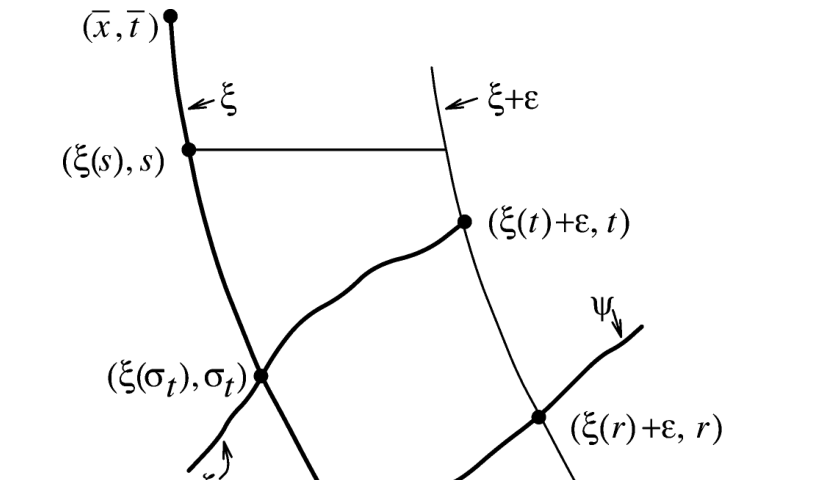
\includegraphics[width=0.6\textwidth]{ch12-fig04-01.png}
\caption{证明\cref{lemma:ch12-振荡估计}所用的特征线几何}
\label{figure:ch12-特征线几何}
\end{figure}

因 $\eta_w(\bar z(t),\bar w(t))<0$，\eqref{align:ch12-H下界}与\eqref{align:ch12-zeta_t}结合蕴含
\begin{align}
H(z(\xi(t)+\varepsilon+,t),w(\xi(t)+\varepsilon+,t),\bar z(t),\bar w(t))
\geqslant[\mu(\bar z(t),\bar w(t))-\lambda(\bar z(t),\bar w(t))]\eta_w(\bar z(t),\bar w(t))[\bar w(\sigma_t)-\bar w(t)].
\label{align:ch12-H下界2}
\end{align}
由于两个特征速度 $\lambda$ 与 $\mu$ 严格分离，$0<t-\sigma_t<c_1\varepsilon$，故\eqref{align:ch12-H下界2}给出
\begin{align}
-\int_r^s H(z(\xi(t)+\varepsilon+,t),w(\xi(t)+\varepsilon+,t),\bar z(t),\bar w(t))\,\mathrm{d}t
\leqslant c_2\varepsilon\sup_{(\tau,s)}|\eta_w(\bar z(\cdot),\bar w(\cdot))|\,NV_{(\tau,s)}\bar w(\cdot),
\label{align:ch12-r段}
\end{align}
其中 $NV$ 表示负（即递减）变差。

接着把 $t$ 限制在区间 $(\tau,r)$。于是 $\zeta_t(\cdot)$ 被 $\tau$-时间线截于 $\zeta_\tau(\tau)\in[\xi(\tau),\xi(\tau)+\varepsilon]$。由\cref{lemma:ch12-迹不增}，
\begin{align}
w(\xi(t)+\varepsilon+,t)=w(\zeta_t(t)+,t)\leqslant w(\zeta_\tau(\tau)+,\tau)=w_0+o(1),\qquad\text{当 }\varepsilon\downarrow0.
\label{align:ch12-tau段w}
\end{align}
另一方面，令 $z_+=\bar z(\tau+)$、$w_+=\bar w(\tau+)$，易见当 $\varepsilon\downarrow0$ 时 $\bar z(t)=z_++o(1)$、$\bar w(t)=w_++o(1)$。因此，将\eqref{align:ch12-H下界}与\eqref{align:ch12-tau段w}结合得
\begin{align}
-\int_\tau^r H(z(\xi(t)+\varepsilon+,t),w(\xi(t)+\varepsilon+,t),\bar z(t),\bar w(t))\,\mathrm{d}t
\leqslant-[\mu(z_+,w_+)-\lambda(z_+,w_+)]\eta_w(z_+,w_+)[w_0-w_+](r-\tau)+o(\varepsilon).
\label{align:ch12-tau段}
\end{align}

现以 $1/\varepsilon$ 乘\eqref{align:ch12-区域积分2}并令 $\varepsilon\downarrow0$。利用\eqref{align:ch12-r段}与\eqref{align:ch12-tau段}，并回忆 $0<r-\tau<c_0\varepsilon$，推得
\begin{align}
\eta(z_1,w_1)-\eta(z_0,w_0)\leqslant c_3\sup_{(\tau,s)}|\eta_w(\bar z(\cdot),\bar w(\cdot))|\,NV_{[\tau,s]}\bar w(\cdot).
\label{align:ch12-eta差}
\end{align}
特别地，$s$ 是满足 $z(\xi(\tau)-,\tau)=z(\xi(\tau)+,\tau)$ 的递增 $\tau$ 序列的极限，而对此类 $\tau$，\eqref{align:ch12-eta差}成立。这进而蕴含 $\eta(z_1,w_1)\leqslant\eta(\bar z(s-),\bar w(s-))$。现对 $t=s$ 应用\eqref{align:ch12-zeta_t}并令 $\varepsilon\downarrow0$，得 $w_1\leqslant\bar w(s-)$。又 $\eta_w<0$、$\eta_z<0$，故 $\bar z(s-)\leqslant z_1$。由\cref{lemma:ch12-迹不增}，$\bar z(s)\leqslant\bar z(s-)$，从而 $z(\xi(s)-,s)=\bar z(s)\leqslant\bar z(s-)\leqslant z_1=z(\xi(s)+,s)$。由于 $s$ 任意，可对 $s=\tau$ 写出这些不等式，即验证了\eqref{align:ch12-夹逼1}。至此\cref{lemma:ch12-迹夹逼}证毕。进而已建立 $z_0\geqslant\bar z(\tau)$，故对一切 $0<\tau<s\leqslant\bar t$，\eqref{align:ch12-eta差}成立。

由\eqref{align:ch12-凸zw}与\eqref{align:ch12-Goursat}得
\begin{align}
\eta(z_1,w_1)-\eta(z_0,w_0)\geqslant z_0-z_1-3\beta\delta(w_1-w_0).
\label{align:ch12-eta凸}
\end{align}
将\eqref{align:ch12-eta差}与\eqref{align:ch12-eta凸}结合，
\begin{align}
z_0-z_1\leqslant 3\beta\delta(w_1-w_0)+c_3\sup_{(\tau,s)}|\eta_w(\bar z(\cdot),\bar w(\cdot))|\,NV_{[\tau,s]}\bar w(\cdot).
\label{align:ch12-z差}
\end{align}
为对一般 $\tau$、$s$ 建立\eqref{align:ch12-振荡1}，只需在 $s-\tau$ 充分小使 $TV_{[\tau,s]}\bar w(\cdot)<2\delta$ 时验证它。对此类 $\tau$、$s$，\eqref{align:ch12-z差}给出初步估计 $z_0-z_1\leqslant c_4\delta$，且事实上对一切 $t\in(\tau,s)$ 有 $z_0-\bar z(t)\leqslant c_4\delta$。但此时因 $|\eta_w(z_0,\bar w(t))|\leqslant5\beta\delta$，\eqref{align:ch12-熵可积}蕴含 $\sup_{(\tau,s)}|\eta_w(\bar z(\cdot),\bar w(\cdot))|\leqslant c_5\delta$。将此估计代入\eqref{align:ch12-z差}，得\eqref{align:ch12-振荡1}，其中 $b=3\beta+c_3c_5$。

最后假设 $\bar w(\tau+)>\bar w(\tau)$，即 $w_+-w_0=\delta_0>0$，并进而验证\eqref{align:ch12-立方1}。固定 $\tau$，选取 $s-\tau$ 充分小使 $TV_{[\tau,s]}\bar w(\cdot)<2\delta_0$，从而 $\delta<2\delta_0$。需改进估计\eqref{align:ch12-tau段}，故将 $t$ 限制在区间 $[\tau,r]$。

由\eqref{align:ch12-凸H}、\eqref{align:ch12-Hz}与\eqref{align:ch12-Hw}，
\begin{align}
H(z(\xi(t)+\varepsilon+,t),w(\xi(t)+\varepsilon+,t),\bar z(t),\bar w(t))
&\geqslant H(z_+,w_0,\bar z(t),\bar w(t))\nonumber\\
&\quad-[\lambda(z_+,w_0)-\lambda(\bar z(t),\bar w(t))][z(\xi(t)+\varepsilon+,t)-z_+]\nonumber\\
&\quad-3\beta\delta[\mu(z_+,w_0)-\lambda(\bar z(t),\bar w(t))][w(\xi(t)+\varepsilon+,t)-w_0].
\label{align:ch12-H上界}
\end{align}
已见当 $\varepsilon\downarrow0$ 时 $\bar z(t)=z_++o(1)$、$\bar w(t)=w_++o(1)$。特别地，当 $\varepsilon$ 小时，由\eqref{align:ch12-混合导数}有 $\lambda(z_+,w_0)-\lambda(\bar z(t),\bar w(t))>0$。进而，若 $\hat\xi(\cdot)$ 表示从任一满足 $\xi(t)<x<\xi(t)+2\varepsilon$ 的点 $(x,t)$ 发出的极小后向 1-特征线，则由\cref{lemma:ch12-迹不增}，当 $\varepsilon\downarrow0$ 时 $z(x-,t)\leqslant z(\hat\xi(\tau)-,\tau)=z_0+o(1)$。另一方面，对 $s\downarrow\tau$，\eqref{align:ch12-振荡1}蕴含 $z_0-z_+\leqslant b\delta_0^2$。因此当 $\varepsilon\downarrow0$ 时 $z(\xi(t)+\varepsilon+,t)\leqslant z_++b\delta_0^2+o(1)$。最后回忆\eqref{align:ch12-tau段w}。综合上述，由\eqref{align:ch12-H上界}推得
\begin{align}
H(z(\xi(t)+\varepsilon+,t),w(\xi(t)+\varepsilon+,t),\bar z(t),\bar w(t))
\geqslant H(z_+,w_0,z_+,w_+)-c_6\delta_0^3+o(1),\qquad\text{当 }\varepsilon\downarrow0.
\label{align:ch12-H上界2}
\end{align}

为估计\eqref{align:ch12-H上界2}的右端，把 $q$ 视为 $(z,\eta)$ 的函数。由链式法则与\eqref{align:ch12-ent流}，推得 $q_\eta=\mu$、$q_{\eta\eta}=\mu_w/\eta_w$。对 $w\in[w_0,w_+]$，$q_{\eta\eta}<0$。故
\begin{align}
H(z_+,w_0,z_+,w_+)\geqslant[\mu(z_+,w_0)-\lambda(z_+,w_+)][\eta(z_+,w_0)-\eta(z_+,w_+)].
\label{align:ch12-Hw0w+}
\end{align}
下一步证明
\begin{align}
\frac{r-\tau}{\varepsilon}\geqslant\frac{1}{\mu(z_0,w_+)-\lambda(z_+,w_+)}+o(1),\qquad\text{当 }\varepsilon\downarrow0.
\label{align:ch12-r比eps}
\end{align}
为看出这一点，从
\begin{align}
\varepsilon=\psi(r)-\xi(r)=\int_\tau^r[\dot\psi(t)-\dot\xi(t)]\,\mathrm{d}t
\leqslant\int_\tau^r[\mu(z(\psi(t)-,t),w(\psi(t)-,t))-\lambda(\bar z(t),\bar w(t))]\,\mathrm{d}t
\label{align:ch12-eps定义}
\end{align}
出发。如上所示，当 $\varepsilon\downarrow0$ 时 $z(\psi(t)-,t)\leqslant z_0+o(1)$。另一方面，从满足 $\xi(t)<x<\psi(t)$ 的点 $(x,t)$ 发出的极大后向 2-特征线 $\zeta(\cdot)$ 将在某 $\sigma\in(\tau,r]$ 处与 $\xi(\cdot)$ 的图像相交，故由\cref{lemma:ch12-迹不增}，$w(x+,t)\leqslant\bar w(\sigma)$。特别地，当 $\varepsilon\downarrow0$ 时 $w(\psi(t)-,t)\leqslant w_++o(1)$。因 $\mu_z>0$、$\mu_w>0$，\eqref{align:ch12-eps定义}蕴含 $\varepsilon\leqslant(r-\tau)[\mu(z_0,w_+)-\lambda(z_+,w_+)+o(1)]$，由此立即得\eqref{align:ch12-r比eps}。

再次以 $1/\varepsilon$ 乘\eqref{align:ch12-区域积分2}，令 $\varepsilon\downarrow0$ 继而令 $s\downarrow\tau$。综合\eqref{align:ch12-r段}、\eqref{align:ch12-H上界2}、\eqref{align:ch12-Hw0w+}与\eqref{align:ch12-r比eps}，得
\begin{align}
\eta(z_+,w_0)-\eta(z_0,w_0)\leqslant\frac{\mu(z_0,w_+)-\mu(z_+,w_0)}{\mu(z_0,w_+)-\lambda(z_+,w_+)}[\eta(z_+,w_0)-\eta(z_+,w_+)]+c_7\delta_0^3.
\label{align:ch12-eta差2}
\end{align}
由\eqref{align:ch12-Goursat}，$\eta(z_+,w_0)-\eta(z_0,w_0)\geqslant z_0-z_+$。\eqref{align:ch12-eta差2}的右端被 $a\delta_0^3$ 界定，因为 $\eta_w=O(\delta_0)$。因此 $z_0-z_+\leqslant a\delta_0^3$。由\eqref{align:ch12-夹逼1}，$\bar z(\tau-)\leqslant z_0$。于是 $\bar z(\tau-)-\bar z(\tau+)\leqslant a\delta_0^3$，即建立了\eqref{align:ch12-立方1}。
\end{proof}

由于总变差可加，立即推得

\begin{corollary}\label{corollary:ch12-局部振荡}
在\eqref{align:ch12-振荡1}（或\eqref{align:ch12-振荡2}）中，$\operatorname{osc}_{[\tau,s]}\bar w(\cdot)$（或 $\operatorname{osc}_{[\tau,s]}\bar z(\cdot)$）可替换为 $\bar w(\cdot)$（或 $\bar z(\cdot)$）在区间 $[\tau,s]$ 内的局部振荡，即由 $\bar w(\cdot)$（或 $\bar z(\cdot)$）在 $[\tau,s]$ 内的最大跳跃度量。特别地，$\bar z(\cdot)$（或 $\bar w(\cdot)$）是阶梯函数，其变差集中在 $\bar w(\cdot)$（或 $\bar z(\cdot)$）的跳跃间断点集上。
\end{corollary}

至此，除\eqref{align:ch12-立方2}是在附加假设 $\bar w(\tau)<\bar w(\tau+)$ 下建立的外，我们已验证了\cref{theorem:ch12-传播主定理}的全部断言。由\cref{lemma:ch12-迹夹逼}，$\bar w(\tau)=w(\xi(\tau)+,\tau)\leqslant w(\xi(\tau)-,\tau)$。另一方面，当 $(\xi(\tau),\tau)$ 是解的局部正则点时，定义\cref{definition:ch12-局部正则}的\ref{item:ch12-局部正则-c1}蕴含 $\bar w(\tau+)=w(\xi(\tau)-,\tau)$。因此，通过建立\cref{theorem:ch12-局部正则存在}，我们将特别证成假设 $\bar w(\tau)<\bar w(\tau+)$。

我们于是转向\cref{theorem:ch12-局部正则存在}的证明。主要工具将是估计\eqref{align:ch12-振荡1}。在下文，$\delta$ 表示上半平面上 $z$ 与 $w$ 振荡的上界。固定上半平面任一点 $(\bar x,\bar t)$，按\cref{section:ch12-解的局部结构}所述并如\cref{figure:ch12-八曲线}所勾勒构造曲线 $\xi_\pm(\cdot)$、$\zeta_\pm(\cdot)$、$\varphi_\pm(\cdot)$ 与 $\psi_\pm(\cdot)$。第一步是验证定义\cref{definition:ch12-局部正则}条件 (a) 中涉及"西"区域 $\mathscr{S}_W$ 的部分。

\begin{lemma}\label{lemma:ch12-西区域}
当 $\theta$ 充分小时，当 $(x,t)$ 穿过由\eqref{align:ch12-区域W}定义的区域 $\mathscr{S}_W$ 趋于 $(\bar x,\bar t)$ 时，$(z(x\pm,t),w(x\pm,t))$ 收敛于 $(z_W,w_W)$，其中令 $z_W=z(\bar x-,\bar t)$、$w_W=w(\bar x-,\bar t)$。
\end{lemma}

\begin{proof}
我们将构造序列 $x_0<x_1<x_2<\cdots<\bar x$，使对每个 $m=0,1,2,\cdots$，
\begin{align}
\operatorname{osc}_{\mathscr{S}_W\cap\{x>x_m\}}z\leqslant(3b\theta)^m\delta,\qquad
\operatorname{osc}_{\mathscr{S}_W\cap\{x>x_m\}}w\leqslant(3b\theta)^m\delta,
\label{align:ch12-西序列}
\end{align}
其中 $b$ 是出现在\eqref{align:ch12-振荡1}中的常数。显然，只要 $3b\theta<1$，\eqref{align:ch12-西序列}即直接给出命题断言。

对 $m=0$，取 $x_0=-\infty$ 即满足\eqref{align:ch12-西序列}。归纳地，设 $x_0<x_1<\cdots<x_{k-1}<\bar x$ 已取定，使对 $m=0,\cdots,k-1$ 成立\eqref{align:ch12-西序列}。现确定 $x_k$。取 $\hat t\in(0,\bar t)$，使 $\bar t-\hat t$ 充分小，$\zeta_-(\hat t)>x_{k-1}$，且 $z(\zeta_-(\tau)\pm,\tau)$ 在区间 $[\hat t,\bar t]$ 上的振荡不超过 $\frac13(3b\theta)^k\delta$。接着在 $(x_{k-1},\zeta_-(\hat t)]$ 中定位 $\hat x$，使 $\zeta_-(\hat t)-\hat x$ 充分小，从而 $w(y-,\hat t)$ 在区间 $(\hat x,\zeta_-(\hat t)]$ 上的振荡同样有界为 $\frac13(3b\theta)^k\delta$。

由 $\varphi_-(\cdot)$ 的构造，从 $\mathscr{S}_W\cap\{x>x_k\}$ 中任一点 $(x,t)$ 发出的极小后向 1-特征线 $\xi(\cdot)$ 保持在 $\varphi_-(\cdot)$ 图像的左侧。同时，当 $(x,t)$ 穿过 $\mathscr{S}_W$ 趋于 $(\bar x,\bar t)$ 时，从它发出的极大后向 2-特征线 $\zeta(\cdot)$ 将趋于某条从 $(\bar x,\bar t)$ 发出的后向 2-特征线，它必位于极小特征线 $\zeta_-(\cdot)$ 之右，或与 $\zeta_-(\cdot)$ 重合。由此，当 $\bar x-x_k$ 充分小时，$\xi(\cdot)$ 必将在某 $t^*\in(\hat t,\bar t)$ 处穿过 $\zeta(\cdot)$ 的图像，而 $\zeta(\cdot)$ 要么在某 $\tilde t\in(\hat t,\bar t)$ 处与 $\zeta_-(\cdot)$ 的图像相交，要么在某 $\tilde x\in(\hat x,\zeta_-(\hat t)]$ 处与 $\hat t$-时间线相交。

由\cref{lemma:ch12-迹不增}与\cref{lemma:ch12-迹夹逼}，
\begin{align}
z(x-,t)\leqslant z(\xi(t^*)-,t^*)=z(\zeta_-(t^*)-,t^*)\leqslant z(\zeta_-(t^*)+,t^*).
\label{align:ch12-西z左}
\end{align}
由\eqref{align:ch12-西序列}在 $m=k-1$ 时及 $\hat t$ 的构造，$w(\xi(\tau)+,\tau)$ 在区间 $[t^*,t]$ 上的振荡不超过 $(3b\theta)^{k-1}\delta+\frac13(3b\theta)^k\delta$，进而被 $2(3b\theta)^{k-1}\delta$ 控制。于是\eqref{align:ch12-振荡1}给出
\begin{align}
z(x+,t)\geqslant z(\xi(t^*)+,t^*)-2b\theta(3b\theta)^{k-1}\delta=z(\zeta_-(t^*)+,t^*)-\frac23(3b\theta)^k\delta.
\label{align:ch12-西z右}
\end{align}
回忆 $z(\zeta_-(\tau)+,\tau)$ 在 $[\hat t,\bar t]$ 上的振荡有界为 $\frac13(3b\theta)^k\delta$，\eqref{align:ch12-西z左}与\eqref{align:ch12-西z右}共同给出 $z$ 在 $m=k$ 时的振荡界\eqref{align:ch12-西序列}。

$w$ 的论证类似：例如设 $\xi(\cdot)$ 与 $\hat t$-时间线相交而非与 $\zeta_-(\cdot)$ 的图像相交。由\cref{lemma:ch12-迹不增}与\cref{lemma:ch12-迹夹逼}，
\begin{align}
w(x+,t)\leqslant w(\zeta(\hat t)+,\hat t)=w(\tilde x+,\hat t)\leqslant w(\tilde x-,\hat t).
\label{align:ch12-西w右}
\end{align}
由\eqref{align:ch12-西序列}在 $m=k-1$ 时，$z(\zeta(\tau)-,\tau)$ 在区间 $[\hat t,t]$ 上的振荡不超过 $(3b\theta)^{k-1}\delta$。于是\eqref{align:ch12-振荡2}蕴含
\begin{align}
w(x-,t)\geqslant w(\zeta(\hat t)-,\hat t)-b\theta(3b\theta)^{k-1}\delta=w(\tilde x-,\hat t)-\frac13(3b\theta)^k\delta.
\label{align:ch12-西w左}
\end{align}
$w$ 在 $m=k$ 时的振荡界\eqref{align:ch12-西序列}现由\eqref{align:ch12-西w右}、\eqref{align:ch12-西w左}及 $\hat t$、$\hat x$ 的构造直接得到。证明完成。
\end{proof}

定义\cref{definition:ch12-局部正则}条件 (a) 中涉及"东"区域 $\mathscr{S}_E$ 的部分，由完全对称的论证验证。下一步是检查条件 (a) 中涉及"南"区域 $\mathscr{S}_S$ 的部分。

\begin{lemma}\label{lemma:ch12-南区域}
当 $\theta$ 充分小时，当 $(x,t)$ 穿过由\eqref{align:ch12-区域S}定义的区域 $\mathscr{S}_S$ 趋于 $(\bar x,\bar t)$ 时，$(z(x\pm,t),w(x\pm,t))$ 趋于常状态 $(z_S,w_S)$。
\end{lemma}

\begin{proof}
与\cref{lemma:ch12-西区域}的证明一样，目标是找到 $t_0<t_1<\cdots<\bar t$，使
\begin{align}
\operatorname{osc}_{\mathscr{S}_S\cap\{t>t_m\}}z\leqslant(4b\theta)^m\delta,\qquad
\operatorname{osc}_{\mathscr{S}_S\cap\{t>t_m\}}w\leqslant(4b\theta)^m\delta,
\label{align:ch12-南序列}
\end{align}
对 $m=0,1,2,\cdots$。对 $m=0$，取 $t_0=0$ 即满足\eqref{align:ch12-南序列}。归纳地，设 $t_0<t_1<\cdots<t_{k-1}<\bar t$ 已取定，使对 $m=0,\cdots,k-1$ 成立\eqref{align:ch12-南序列}，现定位 $t_k$。取 $\hat t\in(t_{k-1},\bar t)$，使 $\bar t-\hat t$ 充分小，$z(\zeta_+(\tau)-,\tau)$、$w(\zeta_+(\tau)+,\tau)$、$z(\zeta_-(\tau)-,\tau)$、$w(\zeta_-(\tau)+,\tau)$ 在区间 $[\hat t,\bar t]$ 上的振荡不超过 $\frac14(4b\theta)^k\delta$。接着在区间 $(\zeta_+(\hat t),\xi_-(\hat t))$ 中定位 $\hat x$ 与 $\tilde x$，使 $\hat x-\zeta_+(\hat t)$ 与 $\xi_-(\hat t)-\tilde x$ 充分小，从而 $z(y-,\hat t)$ 在区间 $(\tilde x,\xi_-(\hat t)]$ 上的振荡与 $w(y+,\hat t)$ 在区间 $[\zeta_+(\hat t),\hat x)$ 上的振荡不超过 $\frac14(4b\theta)^k\delta$。

由于 $\xi_-(\cdot)$ 是极小后向 1-特征线、$\zeta_+(\cdot)$ 是从 $(\bar x,\bar t)$ 发出的极大后向 2-特征线，可找到 $t_k\in(\hat t,\bar t)$，使 $\bar t-t_k$ 充分小，从而对 $\mathscr{S}_S\cap\{t>t_k\}$ 中任一 $(x,t)$ 成立：(a) 从 $(x,t)$ 发出的极小后向 1-特征线 $\xi(\cdot)$ 要么在 $x'\in(\tilde x,\xi_-(\hat t)]$ 处与 $\hat t$-时间线相交，要么在某 $t'\in(\hat t,\bar t)$ 处与 $\xi_-(\cdot)$ 的图像相交；(b) 从 $(x,t)$ 发出的极大后向 2-特征线 $\zeta(\cdot)$ 要么在 $x^*\in[\zeta_+(\hat t),\hat x)$ 处与 $\hat t$-时间线相交，要么在某 $t^*\in(\hat t,\bar t)$ 处与 $\zeta_+(\cdot)$ 的图像相交。然后重复\cref{lemma:ch12-西区域}证明中所用的论证，验证当 $t_k$ 如上确定时，$m=k$ 确满足\eqref{align:ch12-南序列}。证明完成。
\end{proof}

为完成定义\cref{definition:ch12-局部正则}条件 (a) 的验证，还需检查涉及"北"区域 $\mathscr{S}_N$ 的部分。

\begin{lemma}\label{lemma:ch12-北区域}
当 $\theta$ 充分小时，当 $(x,t)$ 穿过由\eqref{align:ch12-区域N}定义的区域 $\mathscr{S}_N$ 趋于 $(\bar x,\bar t)$ 时，$(z(x\pm,t),w(x\pm,t))$ 趋于常状态 $(z_N,w_N)$。
\end{lemma}

\begin{proof}
为确定起见，我们处理\cref{figure:ch12-八曲线}中所示的典型构型，即 $\psi_-\equiv\psi_+$，从而 $\psi_-(\cdot)$ 是一条在 $t=\bar t$ 处强度一般为正的 2-激波，而对 $t>\bar t$ 有 $\varphi_-(t)<\varphi_+(t)$；在此情形，如我们将在\cref{lemma:ch12-北区域出波}中所见，$\lim_{t\downarrow\bar t}z(\varphi_+(t)-,t)=\lim_{t\downarrow\bar t}z(\varphi_+(t)+,t)$，且 $\lim_{t\downarrow\bar t}w(\varphi_+(t)-,t)=\lim_{t\downarrow\bar t}w(\varphi_-(t)+,t)$。对其他可行构型，论证只需稍加修改。

目标是找到 $t_0>t_1>\cdots>\bar t$，使
\begin{align}
\operatorname{osc}_{\mathscr{S}_N\cap\{t<t_m\}}z\leqslant a(ab\theta)^m\delta,\qquad
\operatorname{osc}_{\mathscr{S}_N\cap\{t<t_m\}}w\leqslant 3(ab\theta)^m\delta,
\label{align:ch12-北序列}
\end{align}
对 $m=0,1,2,\cdots$，其中 $a\geqslant1$ 是与 $m$、$\theta$ 无关的常数，将在下文指定。显然，$m=0$ 时取 $t_0=\infty$ 即满足\eqref{align:ch12-北序列}。归纳地，设 $t_0>t_1>\cdots>t_{k-1}>\bar t$ 已取定，使对 $m=0,\cdots,k-1$ 成立\eqref{align:ch12-北序列}，现确定 $t_k$。

选取 $t_k\in(\bar t,t_{k-1})$，使 $t_k-\bar t$ 充分小，从而 $z(\varphi_+(\tau)-,\tau)$ 在区间 $(\bar t,t_k)$ 上的振荡不超过 $a(ab\theta)^{k-1}\delta$，$w(\varphi_+(\tau)-,\tau)$ 在 $(\bar t,t_k)$ 上的振荡有界为 $(ab\theta)^k\delta$，$U(\psi_-(\tau)-,\tau)$ 在 $(\bar t,t_k)$ 上的振荡被 $(ab\theta)^{2k}\delta^2$ 控制。

$w$ 在 $m=k$ 时的振荡界\eqref{align:ch12-北序列}将由\cref{lemma:ch12-西区域}与\cref{lemma:ch12-南区域}证明中所用的程序建立。于是固定 $\mathscr{S}_N\cap\{t<t_k\}$ 中任一 $(x,t)$，考虑从它发出的极大后向 2-特征线 $\zeta(\cdot)$，它在某 $\tilde t\in(\bar t,t_k)$ 处与 $\varphi_+(\cdot)$ 的图像相交。由\cref{lemma:ch12-迹不增}与\cref{lemma:ch12-迹夹逼}，
\begin{align}
w(x+,t)\leqslant w(\zeta(\tilde t)+,\tilde t)=w(\varphi_+(\tilde t)+,\tilde t)\leqslant w(\varphi_+(\tilde t)-,\tilde t).
\label{align:ch12-北w右}
\end{align}
由\eqref{align:ch12-北序列}在 $m=k-1$ 时及 $t_k$ 的构造，$z(\zeta(\tau)-,\tau)$ 在区间 $[\tilde t,t]$ 上的振荡不超过 $2a(ab\theta)^{k-1}\delta$。于是\eqref{align:ch12-振荡2}蕴含
\begin{align}
w(x-,t)\geqslant w(\zeta(\tilde t)-,\tilde t)-2(ab\theta)^k\delta=w(\varphi_+(\tilde t)-,\tilde t)-2(ab\theta)^k\delta.
\label{align:ch12-北w左}
\end{align}
\eqref{align:ch12-北w右}、\eqref{align:ch12-北w左}结合 $w(\varphi_+(\tau)-,\tau)$ 在 $(\bar t,t_k)$ 上的振荡被 $(ab\theta)^k\delta$ 控制这一条件，直接给出 $w$ 在 $m=k$ 时的振荡界\eqref{align:ch12-北序列}。

为推导 $z$ 相应的振荡界，需要完全不同的论证。定义 $\bar U=\lim_{t\downarrow\bar t}U(\psi_-(t)-,t)$，其相应的 Riemann 不变量值为 $(\bar z,\bar w)$，再令 $\Delta z=z-\bar z$、$\Delta w=w-\bar w$。在 $\mathscr{S}_N\cap\{t<t_k\}$ 上，如上所示
\begin{align}
|\Delta w|\leqslant 3(ab\theta)^k\delta.
\label{align:ch12-dw}
\end{align}
我们构造从 $\mathscr{S}_N\cap\{t<t_k\}$ 中任一近似连续点 $(y,t)$ 发出的极小后向 1-特征线 $\xi(\cdot)$，它在某 $t^*\in(\bar t,t_k)$ 处被 $\psi_-(\cdot)$ 的图像截取。于是由\cref{lemma:ch12-迹不增}，$z(y,t)\leqslant z(\xi(t^*)-,t^*)=z(\psi_-(t^*)-,t^*)$，结合 $t_k$ 的选取给出
\begin{align}
\Delta z(y,t)\leqslant c_1(ab\theta)^{2k}\delta^2,
\label{align:ch12-dz}
\end{align}
其中 $c_1$ 是与 $k$、$\theta$ 无关的常数。

现固定 $\mathscr{S}_N\cap\{t<t_k\}$ 中任一近似连续点 $(x,t)$。如上考虑从 $(x,t)$ 发出的极小后向 1-特征线 $\xi(\cdot)$，它在某 $t^*\in(\bar t,t_k)$ 处被 $\psi_-(\cdot)$ 的图像截取，并在区域 $\{(y,\tau):t^*<\tau<t,\ \xi(\tau)<y<\psi_-(\tau)\}$ 上积分守恒律\eqref{align:ch12-系统}。由 Green 定理，
\begin{align}
&\int_x^{\psi_-(t)}[U(y,t)-\bar U]\,\mathrm{d}y\nonumber\\
&\qquad+\int_{t^*}^t\{F(U(\psi_-(\tau)-,\tau))-F(\bar U)-\dot\psi_-(\tau)[U(\psi_-(\tau)-,\tau)-\bar U]\}\,\mathrm{d}\tau\nonumber\\
&\qquad-\int_{t^*}^t\{F(U(\xi(\tau)+,\tau))-F(\bar U)-\lambda(U(\xi(\tau)+,\tau))[U(\xi(\tau)+,\tau)-\bar U]\}\,\mathrm{d}\tau=0.
\label{align:ch12-北积分}
\end{align}
反复应用原书 (7.3.12)，对 $U=U(z,w)$ 得
\begin{align}
U&=\bar U+\Delta z\,R(\bar U)+\Delta w\,S(\bar U)+O(\Delta z^2+\Delta w^2),
\label{align:ch12-U展开}\\
F(U)-F(\bar U)-\lambda(U)[U-\bar U]&=\Delta w[\mu(\bar U)-\lambda(\bar U)]S(\bar U)\nonumber\\
&\quad-\frac12\Delta z^2\lambda_z(\bar U)R(\bar U)-\Delta z\Delta w\lambda_z(\bar U)S(\bar U)+O(\Delta w^2+|\Delta z|^3).
\label{align:ch12-F展开}
\end{align}
还注意到 $w(\xi(\tau)+,\tau)$ 在区间 $(t^*,t)$ 上的振荡有界为 $3(ab\theta)^k\delta$，故由\eqref{align:ch12-振荡1}与\cref{lemma:ch12-迹夹逼}，对任意 $\tau\in(t^*,t)$，
\begin{align}
0\leqslant\Delta z(\xi(\tau)+,\tau)-\Delta z(x,t)\leqslant 3b\theta(ab\theta)^k\delta\leqslant 3(ab\theta)^k\delta.
\label{align:ch12-dz夹逼}
\end{align}
将\eqref{align:ch12-U展开}与\eqref{align:ch12-F展开}代入\eqref{align:ch12-北积分}，再从左端以 $\mathrm{D}z(\bar U)$ 乘所得方程。利用\eqref{align:ch12-riemann归一}、\eqref{align:ch12-dz}、\eqref{align:ch12-dw}、\eqref{align:ch12-真非线性}、\eqref{align:ch12-dz夹逼}及 $t_k$ 的性质，最终得
\begin{align}
\Delta z^2(x,t)\leqslant c(ab\theta)^{2k}\delta^2,
\label{align:ch12-dz平方}
\end{align}
其中 $c$ 是与 $(x,t)$、$k$、$\theta$ 无关的常数。于是选取 $a=\max\{1,2\sqrt c\}$，即达到 $z$ 在 $m=k$ 时的期望界\eqref{align:ch12-北序列}。证明完成。
\end{proof}

为建立定义\cref{definition:ch12-局部正则}的条件 (b)，我们证明

\begin{lemma}\label{lemma:ch12-后向特征极限}
设 $p_\ell(\cdot)$ 与 $p_r(\cdot)$ 是任意两条从 $(\bar x,\bar t)$ 发出的后向 1-特征线，对 $t<\bar t$ 有 $p_\ell(t)<p_r(t)$。若 $\theta$ 充分小，则
\begin{align}
\lim_{t\uparrow\bar t}z(p_\ell(t)+,t)\leqslant\lim_{t\uparrow\bar t}z(p_r(t)-,t),
\label{align:ch12-b限z}\\
\lim_{t\uparrow\bar t}w(p_\ell(t)+,t)\geqslant\lim_{t\uparrow\bar t}w(p_r(t)-,t).
\label{align:ch12-b限w}
\end{align}
\end{lemma}

\begin{proof}
任取序列 $\{(x_n,t_n)\}$，$t_n\uparrow\bar t$（$n\to\infty$），$x_n\in(p_\ell(t_n),p_r(t_n))$ 且充分接近 $p_r(t_n)$，使 $\lim_{n\to\infty}[w(x_n+,t_n)-w(p_r(t_n)-,t_n)]=0$。令 $\zeta_n(\cdot)$ 表示从 $(x_n,t_n)$ 发出的极大后向 2-特征线，它在时刻 $t_n^*$ 与 $p_\ell(\cdot)$ 的图像相交。由\cref{lemma:ch12-迹不增}，$w(x_n+,t_n)\leqslant w(\zeta_n(t_n^*)+,t_n^*)=w(p_\ell(t_n^*)+,t_n^*)$。因 $t_n^*\uparrow\bar t$（$n\to\infty$），这即建立了\eqref{align:ch12-b限w}。

为验证\eqref{align:ch12-b限z}，从另一序列 $\{(x_n,t_n)\}$ 出发，$t_n\uparrow\bar t$，$x_n\in(p_\ell(t_n),p_r(t_n))$，且 $\lim_{n\to\infty}[z(x_n-,t_n)-z(p_\ell(t_n)+,t_n)]=0$。我们构造极小后向 1-特征线 $\xi_n(\cdot)$ 与 $\xi_n^*(\cdot)$，分别从点 $(x_n,t_n)$ 与 $(p_r(t_n),t_n)$ 发出。由极小性，对 $t\leqslant t_n$ 有 $\xi_n(t)\leqslant\xi_n^*(t)\leqslant p_r(t)$。当 $n\to\infty$，$\{\xi_n(\cdot)\}$ 与 $\{\xi_n^*(\cdot)\}$ 一致收敛于无激波的极小 1-分隔线（原书定义 10.3.3 意义下）$\chi(\cdot)$ 与 $\chi^*(\cdot)$，均从 $(\bar x,\bar t)$ 发出，使对 $t\leqslant\bar t$ 有 $\chi(t)\leqslant\chi^*(t)\leqslant p_r(t)$。
特别地，$\dot\chi(\bar t-)\geqslant\dot\chi^*(\bar t-)$，于是
\begin{align}
\lim_{t\uparrow\bar t}\lambda(z(\chi(t)\pm,t),w(\chi(t)\pm,t))\geqslant\lim_{t\uparrow\bar t}\lambda(z(\chi^*(t)\pm,t),w(\chi^*(t)\pm,t)).
\label{align:ch12-lambda序}
\end{align}
以 $\chi(\cdot)$ 与 $\chi^*(\cdot)$ 充当 $p_\ell(\cdot)$ 与 $p_r(\cdot)$，应用\eqref{align:ch12-b限w}得
\begin{align}
\lim_{t\uparrow\bar t}w(\chi(t)+,t)\geqslant\lim_{t\uparrow\bar t}w(\chi^*(t)-,t).
\label{align:ch12-w序}
\end{align}
因 $\lambda_z<0$、$\lambda_w<0$，\eqref{align:ch12-lambda序}与\eqref{align:ch12-w序}共同蕴含
\begin{align}
\lim_{t\uparrow\bar t}z(\chi(t)\pm,t)\leqslant\lim_{t\uparrow\bar t}z(\chi^*(t)\pm,t).
\label{align:ch12-z序}
\end{align}
由\cref{lemma:ch12-迹不增}，$z(\xi_n(t)-,t)$ 与 $z(\xi_n^*(t)-,t)$ 是 $[0,t_n]$ 上的不增函数，故
\begin{align}
\lim_{t\uparrow\bar t}z(\chi(t)\pm,t)\geqslant\lim_{t\uparrow\bar t}z(p_\ell(t)+,t),
\label{align:ch12-z序2}\\
\lim_{t\uparrow\bar t}z(\chi^*(t)\pm,t)\geqslant\lim_{t\uparrow\bar t}z(p_r(t)-,t).
\label{align:ch12-z序3}
\end{align}
于是为完成\eqref{align:ch12-b限z}的证明，还须证明
\begin{align}
\lim_{t\uparrow\bar t}z(\chi^*(t)\pm,t)=\lim_{t\uparrow\bar t}z(p_r(t)-,t).
\label{align:ch12-z等式}
\end{align}

当 $\chi^*\equiv p_r$ 时\eqref{align:ch12-z等式}平凡成立，故取 $t<\bar t$ 时 $\chi^*(t)<p_r(t)$ 的情形。令 $\mathscr{S}=\{(x,t):0\leqslant t<\bar t,\ \chi^*(t)<x<p_r(t)\}$。我们将通过构造 $t_0<t_1<\cdots<\bar t$ 来验证\eqref{align:ch12-z等式}，使
\begin{align}
\operatorname{osc}_{\mathscr{S}\cap\{t>t_m\}}z\leqslant(3b\theta)^m\delta,\qquad
\operatorname{osc}_{\mathscr{S}\cap\{t>t_m\}}w\leqslant(3b\theta)^m\delta,
\label{align:ch12-序序列}
\end{align}
对 $m=0,1,2,\cdots$。对 $m=0$，取 $t_0=0$ 即满足\eqref{align:ch12-序序列}。归纳地，设 $t_0<t_1<\cdots<t_{k-1}<\bar t$ 已取定，使对 $m=0,\cdots,k-1$ 成立\eqref{align:ch12-序序列}，现确定 $t_k$。取 $\hat t\in(t_{k-1},\bar t)$，使 $\bar t-\hat t$ 充分小，$z(\chi^*(\tau)\pm,\tau)$ 与 $w(\chi^*(\tau)-,\tau)$ 在区间 $[\hat t,\bar t]$ 上的振荡不超过 $\frac13(3b\theta)^k\delta$。接着在 $(\chi^*(\hat t),p_r(\hat t))$ 中定位 $\hat x$，使 $\hat x-\chi^*(\hat t)$ 充分小，从而 $z(y+,\hat t)$ 在区间 $[\chi^*(\hat t),\hat x)$ 上的振荡同样有界为 $\frac13(3b\theta)^k\delta$。

由 $\chi^*(\cdot)$ 的构造，若取 $t_k\in(\hat t,\bar t)$ 使 $\bar t-t_k$ 充分小，则从 $\mathscr{S}\cap\{t>t_k\}$ 中任一点 $(x,t)$ 发出的极小后向 1-特征线 $\xi(\cdot)$，要么在某 $t^*\in(\hat t,\bar t)$ 处与 $\chi^*(\cdot)$ 的图像相交，要么在某 $x^*\in(\chi^*(\hat t),\hat x)$ 处与 $\hat t$-时间线相交；而从 $(x,t)$ 发出的极大后向 2-特征线 $\zeta(\cdot)$ 将在某 $\tilde t\in(\hat t,\bar t)$ 处与 $\chi^*(\cdot)$ 的图像相交。

为确定起见，设 $\xi(\cdot)$ 与 $\hat t$-时间线相交。由\cref{lemma:ch12-迹不增}与\cref{lemma:ch12-迹夹逼}，
\begin{align}
z(x-,t)\leqslant z(\xi(\hat t)-,\hat t)=z(x^*-,\hat t)\leqslant z(x^*+,\hat t).
\label{align:ch12-序z左}
\end{align}
由\eqref{align:ch12-序序列}在 $m=k-1$ 时，$w(\xi(\tau)+,\tau)$ 在区间 $[\hat t,t]$ 上的振荡不超过 $(3b\theta)^{k-1}\delta$。于是由\eqref{align:ch12-振荡1}，
\begin{align}
z(x+,t)\geqslant z(\xi(\hat t)+,\hat t)-b\theta(3b\theta)^{k-1}\delta=z(x^*+,\hat t)-\frac13(3b\theta)^k\delta.
\label{align:ch12-序z右}
\end{align}
回忆 $z(y+,\hat t)$ 在 $[\chi^*(\hat t),\hat x)$ 上的振荡与 $z(\chi^*(\tau)+,\tau)$ 在 $[\hat t,\bar t]$ 上的振荡被 $\frac13(3b\theta)^k\delta$ 界定，\eqref{align:ch12-序z左}与\eqref{align:ch12-序z右}共同给出 $z$ 在 $m=k$ 时的界\eqref{align:ch12-序序列}。

$w$ 的论证类似。一方面，由\cref{lemma:ch12-迹不增}与\cref{lemma:ch12-迹夹逼}，
\begin{align}
w(x+,t)\leqslant w(\zeta(\tilde t)+,\tilde t)=w(\chi^*(\tilde t)+,\tilde t)\leqslant w(\chi^*(\tilde t)-,\tilde t).
\label{align:ch12-序w右}
\end{align}
另一方面，考虑到 $z(\zeta(\tau)-,\tau)$ 在区间 $[\tilde t,t]$ 上的振荡被 $(3b\theta)^{k-1}\delta+\frac13(3b\theta)^k\delta$ 界定，而后者小于 $2(3b\theta)^{k-1}\delta$，\eqref{align:ch12-振荡2}给出
\begin{align}
w(x-,t)\geqslant w(\zeta(\tilde t)-,\tilde t)-2b\theta(3b\theta)^{k-1}\delta=w(\chi^*(\tilde t)-,\tilde t)-\frac23(3b\theta)^k\delta.
\label{align:ch12-序w左}
\end{align}
由于 $w(\chi^*(\tau)-,\tau)$ 在 $[\hat t,\bar t]$ 上的振荡不超过 $\frac13(3b\theta)^k\delta$，\eqref{align:ch12-序w右}与\eqref{align:ch12-序w左}共同给出 $w$ 在 $m=k$ 时的界\eqref{align:ch12-序序列}。命题证明完成。
\end{proof}

特别地，可将\cref{lemma:ch12-后向特征极限}用于以 $\xi(\cdot)$ 和/或 $\xi^*(\cdot)$ 充当 $p_\ell(\cdot)$ 或 $p_r(\cdot)$，于是由\cref{lemma:ch12-迹夹逼}，不等式 (12.3.6)$_1$ 与 (12.3.7)$_1$ 分别由\eqref{align:ch12-b限z}与\eqref{align:ch12-b限w}推出。这样我们已验证定义\cref{definition:ch12-局部正则}的条件 (b)$_1$。条件 (b)$_2$ 可由完全对称的论证验证。

还需检查定义\cref{definition:ch12-局部正则}的条件 (c)。只需验证 (c)$_1$，因为 (c)$_2$ 由类似论证直接得到。在激波情形 $\varphi_-\equiv\varphi_+$，所需不等式 $z_W\leqslant z_N$ 与 $w_W\geqslant w_N$ 是\cref{lemma:ch12-迹夹逼}的直接推论。故只需考虑稀疏波情形。

\begin{lemma}\label{lemma:ch12-北区域出波}
设对 $t>\bar t$ 有 $\varphi_-(t)<\varphi_+(t)$。当 $\theta$ 充分小时，当 $(x,t)$ 在区域 $\mathscr{W}=\{(x,t):t>\bar t,\ \varphi_-(t)<x<\varphi_+(t)\}$ 中趋于 $(\bar x,\bar t)$ 时，$w(x\pm,t)$ 趋于 $w_W$。进而，对任意 1-特征线 $p_\ell(\cdot)$、$p_r(\cdot)$，若对 $t>\bar t$ 有 $\varphi_-(t)\leqslant p_\ell(t)\leqslant p_r(t)\leqslant\varphi_+(t)$，则 (12.3.8)$_1$ 成立。
\end{lemma}

\begin{proof}
考虑穿过 $\mathscr{W}$ 趋于 $(\bar x,\bar t)$ 的点 $(x,t)$。从 $(x,t)$ 发出的极大后向 2-特征线 $\zeta(\cdot)$ 在 $\zeta(\bar t)$ 处被 $\bar t$-时间线截取，该点从下方趋于 $\bar x$。由\cref{lemma:ch12-迹不增}易见 $\limsup w(x\pm,t)\leqslant w_W$。为验证命题断言，须证明 $\liminf w(x\pm,t)=w_W$。我们用反证法，假设 $\liminf w(x\pm,t)=w_W-\beta$，$\beta>0$。

取 $\hat t>\bar t$，使 $\hat t-\bar t$ 充分小，
\begin{align}
w_W-2\beta<w(x\pm,t)\leqslant w_W+\beta,\qquad \bar t<t<\hat t,\ \varphi_-(t)<x<\varphi_+(t),
\label{align:ch12-w界}
\end{align}
此外，函数 $z(\varphi_-(t)\pm,t)$ 与 $w(\varphi_-(t)\pm,t)$ 在区间 $(\bar t,\hat t)$ 上的振荡不超过 $\frac12\beta$。

我们考虑从任一点 $(\tilde x,\tilde t)$（$\bar t<\tilde t<\hat t$，$\varphi_-(\tilde t)<\tilde x<\varphi_+(\tilde t)$）发出的极大后向 2-特征线 $\zeta(\cdot)$，它在某 $t^*\in(\bar t,\hat t)$ 处与 $\varphi_-(\cdot)$ 的图像相交。我们证明，当 $\theta$ 充分小（与 $\beta$ 无关）时，有
\begin{align}
w(\zeta(t)-,t)-w(\tilde x-,\tilde t)\leqslant\frac{\beta}{4},\qquad t^*<t<\tilde t.
\label{align:ch12-zeta衰减}
\end{align}
事实上，若\eqref{align:ch12-zeta衰减}不成立，则可找到 $t_1$、$t_2$，$t^*<t_1<t_2\leqslant\tilde t$，且 $t_2-t_1$ 任意小，使
\begin{align}
|z(\zeta(t_1)\pm,t_1)-z(\zeta(t_2)\pm,t_2)|>\frac{\beta}{4b\theta}.
\label{align:ch12-矛盾}
\end{align}
特别地，若 $\xi_1(\cdot)$ 与 $\xi_2(\cdot)$ 表示从点 $(\zeta(t_1),t_1)$ 与 $(\zeta(t_2),t_2)$ 发出的极小后向 1-特征线，从而它们必穿过点 $(\bar x,\bar t)$，则 $t_1$ 与 $t_2$ 可取充分接近，使
\begin{align}
0\leqslant\int_0^{t_1}\lambda(z(\xi_2(t)-,t),w(\xi_2(t)-,t))\,\mathrm{d}t-\int_0^{t_1}\lambda(z(\xi_1(t)-,t),w(\xi_1(t)-,t))\,\mathrm{d}t\leqslant\beta t_0.
\label{align:ch12-积分lambda}
\end{align}
由\eqref{align:ch12-w界}，对一切 $t\in(\bar t,t_1)$ 有 $|w(\xi_2(t)-,t)-w(\xi_1(t)-,t)|<3\beta$。又由\cref{lemma:ch12-迹不增}、\eqref{align:ch12-振荡1}与\eqref{align:ch12-w界}，对 $(\bar t,t_1)$ 中几乎所有 $t$，
\begin{align}
\begin{cases}
z(\zeta(t_1)-,t_1)\leqslant z(\xi_1(t)-,t)=z(\xi_1(t)+,t)\leqslant z(\zeta(t_1)+,t_1)+3\beta b\theta,\\
z(\zeta(t_2)-,t_2)\leqslant z(\xi_2(t)-,t)=z(\xi_2(t)+,t)\leqslant z(\zeta(t_2)+,t_2)+3\beta b\theta.
\end{cases}
\label{align:ch12-z夹}
\end{align}
现显然，当 $\theta$ 充分小时，\eqref{align:ch12-z夹}使\eqref{align:ch12-矛盾}与\eqref{align:ch12-积分lambda}不相容。这就提供了验证\eqref{align:ch12-zeta衰减}所需的矛盾。

由\cref{lemma:ch12-西区域}及 $\hat t$ 的构造，
\begin{align}
\lim_{t\downarrow\bar t}z(\varphi_-(t)-,t)=z_W,\qquad \lim_{t\downarrow\bar t}w(\varphi_-(t)-,t)=w_W,
\label{align:ch12-phi-极限}\\
|z(\varphi_-(t^*)-,t^*)-z_W|\leqslant\frac{\beta}{2},\qquad |w(\varphi_-(t^*)-,t^*)-w_W|\leqslant\frac{\beta}{2}.
\label{align:ch12-phi-夹}
\end{align}
下一步建立估计
\begin{align}
|z(\varphi_-(t^*)-,t^*)-\lim_{t\downarrow t^*}z(\zeta(t)-,t)|\leqslant a\beta,
\label{align:ch12-z估计}
\end{align}
其中 $a$ 是与 $\theta$、$\beta$ 无关的常数。令
\begin{align}
\lim_{t\downarrow\bar t}z(\varphi_-(t)+,t)=z_W+\gamma,
\label{align:ch12-zphi+}
\end{align}
$\gamma\geqslant0$。取 $t_3\in(t^*,\hat t)$ 与 $x_3\in(\varphi_-(t_3),\varphi_+(t_3))$，使 $x_3-\varphi_-(t_3)$ 充分小，从而
\begin{align}
|z(x_3\pm,t_3)-z_W-\gamma|\leqslant\beta.
\label{align:ch12-x3}
\end{align}
再选 $t_3-t^*$ 充分小，从点 $(x_3,t_3)$ 发出的极小后向 1-特征线 $\xi(\cdot)$ 将在任意接近 $t^*$ 的时刻 $t_4$ 与 $\zeta(\cdot)$ 的图像相交。由\cref{lemma:ch12-迹不增}，$z(\zeta(t_4)-,t_4)\geqslant z(x_3-,t_3)$。另一方面，由\eqref{align:ch12-w界}，\cref{lemma:ch12-振荡估计}蕴含 $z(\zeta(t_4)+,t_4)\leqslant z(x_3+,t_3)+3b\theta\beta$。于是，当 $6b\theta\leqslant1$ 时，$|z_W+\gamma-\lim_{t\downarrow t^*}z(\zeta(t)-,t)|\leqslant\frac32\beta$。结合\eqref{align:ch12-phi-夹}，得
\begin{align}
|z(\varphi_-(t^*)-,t^*)-\lim_{t\downarrow t^*}z(\zeta(t)-,t)|\leqslant 2\beta+\gamma.
\label{align:ch12-z估计2}
\end{align}
因此，为验证\eqref{align:ch12-z估计}，还须证明 $\gamma\leqslant c\beta$。

特征线 $\xi(\cdot)$ 位于 $\varphi_-(\cdot)$ 之右并穿过点 $(\bar x,\bar t)$，故 $\dot\varphi_-(\bar t+)\leqslant\dot\xi(\bar t+)$。由\eqref{align:ch12-phi-极限}、\eqref{align:ch12-zphi+}、原书 (8.2.1)、(8.2.2)、(7.3.12)、(8.2.3) 与\eqref{align:ch12-riemann归一}，得
\begin{align}
\dot\varphi_-(\bar t+)=\lambda(z_W,w_W)+\frac12\lambda_z(z_W,w_W)\gamma+O(\gamma^2).
\label{align:ch12-phidot}
\end{align}
为估计 $\dot\xi(\bar t+)=\lim_{t\downarrow\bar t}\lambda(z(\xi(t)-,t),w(\xi(t)-,t))$，回忆 $\lambda_z<0$、$\lambda_w<0$、$z(\xi(t)-,t)\geqslant z(x_3-,t_3)\geqslant z_W+\gamma-\beta$、$w(\xi(t)-,t)\geqslant w_W-2\beta$，故
\begin{align}
\dot\xi(\bar t+)\leqslant\lambda(z_W+\gamma-\beta,w_W-2\beta)=\lambda(z_W,w_W)+\lambda_z(z_W,w_W)\gamma+O(\beta+\gamma^2).
\label{align:ch12-xidot}
\end{align}
因此 $\gamma=O(\beta)$，\eqref{align:ch12-z估计}由\eqref{align:ch12-z估计2}得到。

由\cref{lemma:ch12-振荡估计}，\eqref{align:ch12-z估计}给出
\begin{align}
w(\varphi_-(t^*)-,t^*)-\lim_{t\downarrow t^*}w(\zeta(t)-,t)\leqslant ab\theta\beta.
\label{align:ch12-w估计}
\end{align}
于是，若 $\theta\leqslant(8ab)^{-1}$，则\eqref{align:ch12-zeta衰减}、\eqref{align:ch12-w估计}与\eqref{align:ch12-phi-夹}共同蕴含，对 $\mathscr{W}\cap\{t<\hat t\}$ 中一切 $(\tilde x,\tilde t)$，有 $w_W-w(\tilde x-,\tilde t)\leqslant\frac78\beta$。这就对假设 $\liminf w(x\pm,t)=w_W-\beta$（$\beta>0$）提供了期望的矛盾，从而验证了当 $(x,t)$ 穿过 $\mathscr{W}$ 趋于 $(\bar x,\bar t)$ 时 $w(x\pm,t)$ 趋于 $w_W$。

现把注意力集中到 $\varphi_+(\cdot)$。已有 $\lim_{t\downarrow\bar t}w(\varphi_+(t)-,t)=w_W$、$\lim_{t\downarrow\bar t}z(\varphi_+(t)+,t)=z_N$、$\lim_{t\downarrow\bar t}w(\varphi_+(t)+,t)=w_N$。令 $z_0=\lim_{t\downarrow\bar t}z(\varphi_+(t)-,t)$。则 $\lambda(z_0,w_W)\geqslant\dot\varphi_+(\bar t+)\geqslant\lambda(z_N,w_N)$。目标是证明 $\dot\varphi_+(\bar t+)=\lambda(z_0,w_W)$，从而推得 $z_N=z_0$、$w_N=w_W$。我们考虑从点 $(\varphi_+(t_5),t_5)$（$t_5-\bar t$ 很小）发出的极小后向 1-特征线 $\xi(\cdot)$。当 $\xi\equiv\varphi_+$ 时断言 $z_N=z_0$、$w_N=w_W$ 显然成立，故设 $t\in(\bar t,t_5)$ 时 $\xi(t)<\varphi_+(t)$。于是 $|w(\xi(t)+,t)-w_W|$ 在 $(\bar t,t_5)$ 上很小。进而，由\cref{lemma:ch12-振荡估计}，$z(\xi(t)+,t)$ 在区间 $(\bar t,t_5)$ 上的振荡很小，故该函数取接近 $z_0$ 的值。因此 $t_5-\bar t$ 充分小使 $\dot\xi(\bar t+)$ 任意接近 $\lambda(z_0,w_W)$。因 $\dot\xi(\bar t+)\leqslant\dot\varphi_+(\bar t+)$，推得 $\dot\varphi_+(\bar t+)\geqslant\lambda(z_0,w_W)$，从而必有 $\dot\varphi_+(\bar t+)=\lambda(z_0,w_W)$。

现考虑任一从 $(\bar x,\bar t)$ 发出的前向 1-特征线 $\chi(\cdot)$，对 $t>\bar t$ 有 $\varphi_-(t)\leqslant\chi(t)\leqslant\varphi_+(t)$。由于 $\lim_{t\downarrow\bar t}w(\chi(t)-,t)$ 与 $\lim_{t\downarrow\bar t}w(\chi(t)+,t)$ 取同一值 $w_W$，$\lim_{t\downarrow\bar t}z(\chi(t)-,t)$ 与 $\lim_{t\downarrow\bar t}z(\chi(t)+,t)$ 也必取同一值，记为 $z_\chi$。特别地，$\dot\chi(\bar t+)=\lambda(z_\chi,w_W)$。因此，若 $p_\ell(\cdot)$ 与 $p_r(\cdot)$ 是任意两条 1-特征线，对 $t>\bar t$ 有 $\varphi_-(t)\leqslant p_\ell(t)\leqslant p_r(t)\leqslant\varphi_+(t)$，则不等式 $\dot\varphi_-(\bar t+)\leqslant\dot p_\ell(\bar t+)\leqslant\dot p_r(\bar t+)\leqslant\dot\varphi_+(\bar t+)$ 对 $\bar t$ 处传播速度排序，结合 $\lambda_z<0$，共同蕴含 (12.3.8)$_1$。证明完成。
\end{proof}

至此，我们已完成局部正则性\cref{theorem:ch12-局部正则存在}的证明，也完成了 Riemann 不变量沿极值后向特征线传播定律\cref{theorem:ch12-传播主定理}的证明。这些将作为推导解大时间行为先验估计的主要工具。

从今往后，我们的解将通过定义 $(z(x,t),w(x,t))=(z_S,w_S)$ 而在 $(-\infty,\infty)\times(0,\infty)$ 上归一化，即在 $(x,t)$ 处取"南"极限。于是解在任一类空曲线上的迹，定义为归一化 $(z,w)$ 在该曲线上的限制。特别地，这使 $(z,w)$ 沿从任一点 $(\bar x,\bar t)$ 发出的极小后向 1-特征线与极大后向 2-特征线的迹，在 $(0,\bar t]$ 上从左连续。

\end{document}
